%% LaTeX-Beamer template for KIT design
%% by Erik Burger, Christian Hammer
%% title picture by Klaus Krogmann
%%
%% version 2.1
%%
%% mostly compatible to KIT corporate design v2.0
%% http://intranet.kit.edu/gestaltungsrichtlinien.php
%%
%% Problems, bugs and comments to
%% burger@kit.edu

\documentclass[18pt]{beamer}

%% SLIDE FORMAT

% use 'beamerthemekit' for standard 4:3 ratio
% for widescreen slides (16:9), use 'beamerthemekitwide'

\usepackage{templates/beamerthemekit}
% \usepackage{templates/beamerthemekitwide}

%% TITLE PICTURE

% if a custom picture is to be used on the title page, copy it into the 'logos'
% directory, in the line below, replace 'mypicture' with the 
% filename (without extension) and uncomment the following line
% (picture proportions: 63 : 20 for standard, 169 : 40 for wide
% *.eps format if you use latex+dvips+ps2pdf, 
% *.jpg/*.png/*.pdf if you use pdflatex)

%\titleimage{mypicture}

%% TITLE LOGO

% for a custom logo on the front page, copy your file into the 'logos'
% directory, insert the filename in the line below and uncomment it

%\titlelogo{mylogo}

% (*.eps format if you use latex+dvips+ps2pdf,
% *.jpg/*.png/*.pdf if you use pdflatex)

%% TikZ INTEGRATION

% use these packages for PCM symbols and UML classes
% \usepackage{templates/tikzkit}
% \usepackage{templates/tikzuml}

% the presentation starts here

\title[Specification presentation]{Dynamic scheduler for scientific simulations}
\subtitle{Final presentation}
\author{Kai Bittner, Ard Kastrati, Fabio Broghammer, Jan Ellmers, David Krenz, Benjamin-Philip Roth}

\institute{Steinbuch Centre for Computing (SCC)}

% Bibliography

\usepackage[citestyle=authoryear,bibstyle=numeric,hyperref,backend=biber]{biblatex}
\addbibresource{templates/example.bib}
\bibhang1em

\begin{document}

% change the following line to "ngerman" for German style date and logos
\selectlanguage{english}

%title page
\begin{frame}
\titlepage
\end{frame}

%table of contents
\begin{frame}{Outline}
\tableofcontents
\end{frame}

\section{Overview}
\begin{frame}{Overview}

\centerline{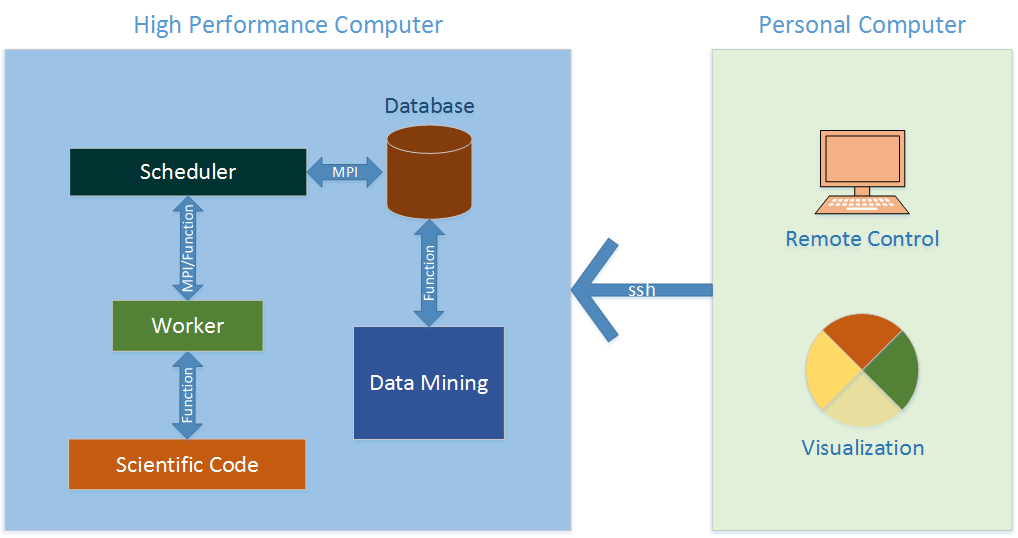
\includegraphics[scale=0.43]{images/overview}}
\end{frame}


	\begin{frame}{Master-Worker}
		\centerline{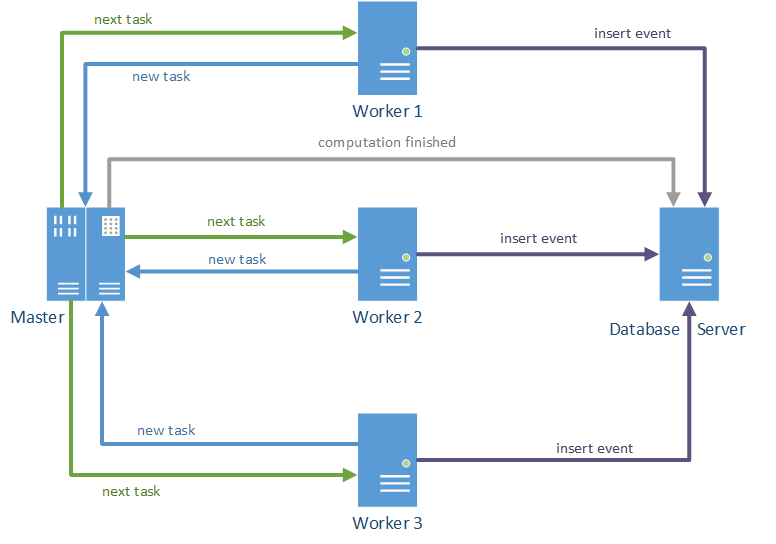
\includegraphics[scale=0.5]{images/master}}
	\end{frame}
	\begin{frame}{Task Stealing}
		\centerline{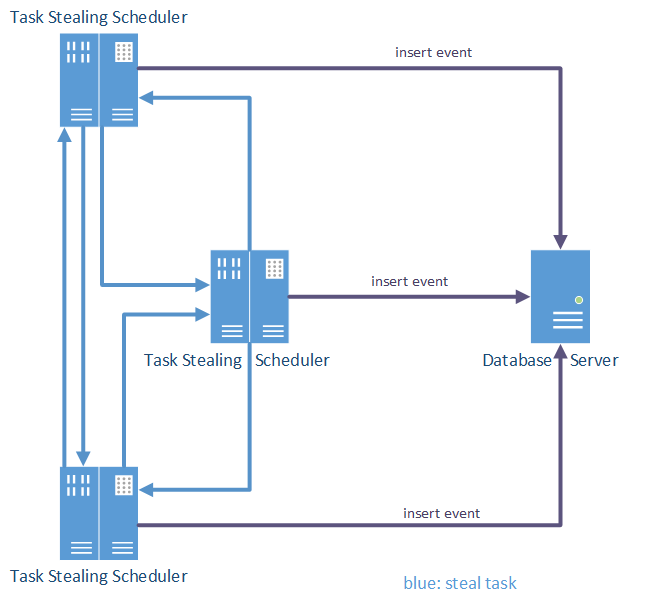
\includegraphics[scale=0.5]{images/taskstealing}}
	\end{frame}

	\begin{frame}{Scheduling Strategies}
	\begin{minipage}[]{.7\textwidth}%
			\begin{itemize}
		\item<2-> Non-statistical
		\begin{itemize}
			\item<3-> First In-First Out (FIFO)
			\item<4-> Last In-Fist Out (LIFO)
		\end{itemize}
		\item<5-> Statistical
		\begin{itemize}
			\item<6-> Shortest Job First (SJF)
			\item<7-> Longest Job First (LJF)
		\end{itemize}
		\item<8-> Standardized interface 
			\begin{itemize}
				\item<9-> simple to include new strategies
			\end{itemize}					
		\end{itemize}
\end{minipage}%
\begin{minipage}[]{.3\textwidth}%
  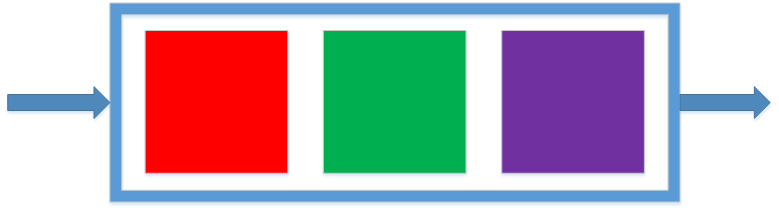
\includegraphics[width=\textwidth]{images/fifo}%
\end{minipage}		
		
	\end{frame}
	\begin{frame}{Master-Worker vs. Task Stealing}
		\begin{itemize}
			\item<2-> Master-Worker
				\begin{itemize}
					\item<3-> fast standard c++ implementation
					\item<4-> dynamic size
					\item<5-> easy to switch between scheduling strategies at runtime	
				\end{itemize}
			
			\item<6-> Task stealing
					\begin{itemize}
						\item<7-> custom implementation inside a MPI-Window
					\end{itemize}
			
		\end{itemize}
	\end{frame}

\end{document}
